\documentclass{book}
\synctex=1
\usepackage[default]{fontsetup}
\newfontfamily\newcmgreekguillemots[CharacterVariant=4]{NewCM10-Book.otf}
\newfontfamily\devfont[Script=Devanagari,Language=Marathi]{NewCM10Devanagari-Book.otf}
\newcommand\leftgrquotes{\char"201C}
\newcommand\rightgrquotes{\char"201E}
\usepackage{graphicx,fullpage,supertabular}
\AtBeginDocument{\def\varnothing{\char"2300}\def\emptyset{\char"2205}}
\begin{document}


  \begin{center}
    {\LARGE The \texttt{fontsetup} package}\\[1ex]
    \textit{by}\\[1ex]
    {\large Antonis Tsolomitis}\\
University of the Aegean\\ Department of Mathematics\\[1ex]
	  \textsc{1} November \textsc{2024}\\[1ex]
	  Version 2.3.0, \textsc{gpl3}
  \end{center}

This package is a simple wrapper-type package that makes the setup of fonts easy and
  quick for XeLaTeX and LuaLaTeX. You just load the package using one of the supported
  fonts as an option.

  The target is to provide easy access to fonts with a matching Mathematics font available in
  TeX distributions plus a few commercial if available.

  The package will include more font combinations in the future, however there are
  some restrictions. The fonts must have some commercial-level quality and must support
  Mathematics.

  Version 2.1.0 adds commands for accessing the Aegean Numbers (U10100-U1013F) for
  the default and olddefault options as described in Appendix~\ref{AegeanNumbers}.
  
  Version 2.0 has restructured the files of the package to a better and easier to be maintained
  way. Many thanks go to {\devfont निरंजन} (Niranjan) for helping me with this.
  
  Starting with version 1.01 the package is split in two; the main package called ``fontsetup''
  and the fontsetup-nonfree package that contains the support and sample files for the
  non-free fonts. This facilitates the installation for users of texlive since the latter does not
  install the support for non-free fonts. For a user who wants to install the support for
  non-free fonts (Cambria, Lucida, Adobe-Minion, MS-Garamond, and Linotype-Palatino) it can be
  easily done following the guide for the contrib repository here:

  https://contrib.texlive.info

  The main package will load the style files for the nonfree fonts if the fontsetup-nonfree
  package is installed; that is, there is no other package that the user needs to
  load in the TeX file.
  
  The options (in alphabetic order after the default option) are as follows:

  \begin{description}
  \item[default] Loads the NewComputerModern fonts (in Book weight),
    which is an assembly of cm fonts plus
    more fonts to support Greek (cbgreek) and Cyrillic languages. It also provides
    \begin{itemize}
    \item the option ``upint'' for switching to upright integrals in mathmode.
    \item the option ``varnothing'' for changing the default symbol for
      the empty set ($\emptyset$) to the \verb|\varnothing| symbol ($\varnothing$) in mathmode.
      \item the option ``newcmbb'' for selecting the NewCM blackboard bold instead of the AMS one.
      \item commands to access prosgegrammeni instead of ypogegrammeni for capitals and small
        capitals, by writing \verb|\textprosgegrammeni{<text>}| or \verb|{\prosgegrammeni <text>}|.
      \item commands to access 4th and 6th century bce Greek by writing
        \verb|\textivbce{<text>}| or \verb|{\ivbce <text>}| and
        \verb|\textvibce{<text>}| or \verb|{\vibce <text>}|. For example, write
        \verb|\textivbce{ΕΠΙΚΟΥΡΟΣ}| to get \textivbce{ΕΠΙΚΟΥΡΟΣ}.
      \item commands to access Sans Greek (upright and oblique) in math mode although these are
        not included in the unicode standard. The commands follow the unicode-math.sty notation, so
        to get $\msansLambda$ and $\mitsanspi$ you write \verb|$\msansLambda$| and \verb|$\mitsanspi$|.
      \item commands to access the Ancient Greek Numbers (Unicode u10140--u1018E)
        documented in the Appendix
      \item commands to access the negation of uniform convergence symbols \verb|\nrightrightarrows|
        for $\nrightrightarrows$ and \verb|\nleftleftarrows| for $\nleftleftarrows$, and
        1-1 and onto functions: \verb|\twoheadhookrightarrow| for $\twoheadhookrightarrow$ and
        \verb|\twoheadhookleftarrow| for $\twoheadhookleftarrow$.
      \item command \verb|\convolution| to access the new convolution operator $\convolution$
        (check the documentation of NewCM fonts).
      \item commands to access the IPA symbols. These are \verb|\ipatext| and
        \verb|\textipa{...}| to select the fonts
        for IPA symbols locally. Compare \textipa{ðŋβθχ}
        (produced with \verb|\textipa{ðŋβθχ}|) with ðŋβθχ.
        \verb|\textoldipa| is also available (check the documentation of
        the NewComputerModern family).
      \item If the xgreek package is loaded before fontsetup this will be detected and the package
        will load the fonts with correct anoteleia, greek guillemots and proper apostrophe for
        Greek. It will also enable the commands \verb|\leftgrquotes| and \verb|\rightgrquotes| for proper
        quotes inside quotes. For an example, writing

        \verb|«φώναζε: \leftgrquotes απ' έξω την προπαίδεια\rightgrquotes»· σαν εκδίκηση ακουγόταν\ldots|

        will give
        
\begin{center}
{\newcmgreekguillemots  «φώναζε: \leftgrquotes απ' έξω την προπαίδεια\rightgrquotes»· σαν εκδίκηση ακουγόταν\ldots}
\end{center}
For more information and references see the documentation of the
NewComputerModern font family.
      \item commands to access ``up'' versions of Greek letters for Chemistry: Use \verb|chemalpha|,
        \verb|\chembeta|, \verb|\chemgamma| etc and similarly for uppercase (\verb|\chemAlpha| etc).
        For example, \verb|\chembeta-gucan| gives ``\chembeta-gucan'' and \verb|\chemkappa-component|
        gives ``\chemkappa-component''.
      \item commands for Medieval Latin and Uncial Greek:
        use \verb|{\uncial text}| or \verb|\textuncial{text}|.
      \item commands to access the Aegean Numbers (U10100 to U1013F) as described in
        Appendix~\ref{AegeanNumbers}.
    \end{itemize}
  \item[olddefault] Loads the NewComputerModern fonts (in Regular weight)
    similarly to the default option.
  \item[sansdefault] Loads the NewComputerModern Sans Serif fonts (in Regular weight)
    similarly to the default option with Sans Math.
  \item[cambria] Loads the Cambria fonts of Microsoft. These must be already installed
    as a system font (in \verb|C:\Windows\Fonts| in MS-Windows, in \verb|/home/user/.fonts/| in Linux
    or elsewhere by the system administratior). This option works only if
    fontsetup-nonfree is installed.
  \item[concrete] Loads the Concrete fonts from the \texttt{cmu} package with Concrete-Math
    font for mathematics.
  \item[ebgaramond] Loads the EB-Garamond fonts with Garamond-Math and complements them with
    Ysabeau for Sans.
    \item[erewhon] Loads the Erewhon fonts with Erewhon-Math.
    \item[euler] Loads the Concrete fonts with the Euler-Math for Mathematics. This option replaces
      the older option \texttt{neoeuler} which was using the neoeuler font. This font has continued
      its development as Euler-Math. I want to thank Shyam Sundar for helping with the
      proper setup of the support for the math font and it's fallback to TeX Gyre Pagella for
      glyphs not yet covered by Euler-Math. \textit{Important notice}: the fallback mechanism is slow. Expect
	delays at each run.
    \item[fira] Loads the Fira family, a sans-serif font.
    \item[gfsartemisia] Loads the GFSArtemisia, a font family designed to be used
      as a Times replacement. The Mathematics is from stix2 but latin
      and greek letters are substituted from GFSArtemisia to provide a better match.
    \item[gfsdidotclassic] Uses the GFSDidotClassic for Greek with GFSPorson for italic.
      The latin part is URW garamond. The Mathematics is from Garamond-Math but the greek
      letters are substituted from GFSDidotClassic to provide a better match. Notice that
      the Bold versions of the Greek fonts are faked using fontspec mechanism as
      the Greek part does not have bold versions.
    \item[gfsdidot] Loads the GFSDidot fonts. NewCMMath-Book is the Mathematics font, but latin
      and greek letters are substituted from GFSdidot to provide a better match.
    \item[gfsneohellenic] Loads the GFSNeohellenic family with GFSNeohellenic-Math.
    \item[kerkis] Loads the kerkis font family and texgyrebonum-math.
    \item[libertinus] Loads the Libertinus and LibertinusMath fonts.
    \item[lucida] Loads the Lucida font family if available (a commercial font). This option works only if
    fontsetup-nonfree is installed.
    \item[minion] Loads the MinionPro family. To install it, find the fonts MinionPro and
      MyriadPro from the installation of Adobe PDF Reader and install the fonts to your system
      (in \verb|C:\Windows\Fonts| in MS-Windows, in \verb|/home/user/.fonts/| in Linux
      or elsewhere by the system administratior). Moreover, install the supplied
      fspmnscel.otf as a system font to have access to Greek small caps.
      Mathematics is from stix2
      with letters replaced from MinionPro. Sans is MyriadPro. This option works only if
    fontsetup-nonfree is installed.
    \item[msgaramond] Loads the MS-Garamond fonts. These must be system installed
      (in \verb|C:\Windows\Fonts| in MS-Windows, in \verb|/home/user/.fonts/| in Linux
      or elsewhere by the system administratior). Mathematics is from
      Garamond-Math with letters replaced
      from MS-Garamond. This option works only if
    fontsetup-nonfree is installed.
    \item[neoeuler] This option is preserved for backwards compatibility. See option \texttt{euler}.
\item[oldstandard] Loads the OldStandard fonts. Mathematics is from
      OldStandard-Math.
    \item[palatino] Loads the Linotype Palatino Fonts available from some versions of Windows.
      Thefonts must be system installed (in \verb|C:\Windows\Fonts| in MS-Windows,
      in \verb|/home/user/.fonts/| in Linux or elsewhere by the system administratior). The supplied
      fsplpscel.otf must be also
      system-installed to allow access to Greek small caps.
      Mathematics font is texgyrepagella-math. This option works only if
    fontsetup-nonfree is installed.
  \item[stixtwo] Loads the stix2 fonts, a Times-type font.
    \item[talos] Loads the NewCM Book weight with the Greek cult font Talos.
    \item[times] Loads the FreeSerifb fonts, a Times font and stix2 for Mathematics
      with letters replaced from FreeSerifb.
    \item[xcharter] Loads the XCharter fonts and the XCharter-Math font. The option \verb|upint| is provided for upright style integrals. The sans fonts are CabinCondensed and the mono fonts are
      Inconsolatazi4.
  \end{description}

  You do not need to load \verb|fontspec|. This, as well as \verb|unicode-math|, are
  automatically loaded. A minimal file is
\begin{verbatim}
  \documentclass{article}
  \usepackage[default]{fontsetup}
  \begin{document}
  ...
  \end{document}
\end{verbatim}

The switch to another font is trivial. You just change the option of \verb|fontsetup|
to another among the supported ones.


\bigskip

\textbf{Summary of installation steps to support all fonts}

%\medskip
%
%For accessing the free fonts there is nothing to install (provided
%you have a full installation of TeX system) unless you want to access
%the \verb|neoeuler| option. For this you have to install
%\verb|euler.otf| in your TeX tree from
%  here: \verb|https://github.com/khaledhosny/euler-otf|

\medskip

To access commercial fonts supported by this package check the
documentation of the fontsetup-nonfree package.


\medskip

You can indeed suggest a new combination of fonts and I will add them. However, I do
reserve the right to reject them if the font quality is bad or if Mathematics is not supported
with a matching font.

Samples for the free fonts follow. Samples for the nonfree fonts can be found in

\noindent fontsetup-nonfree/doc/fontsetup-nonfree-doc.pdf

\newpage


\begin{center}
{\Large NewComputerModern fonts (Book weight): option \verb|default|}\\[1cm] 
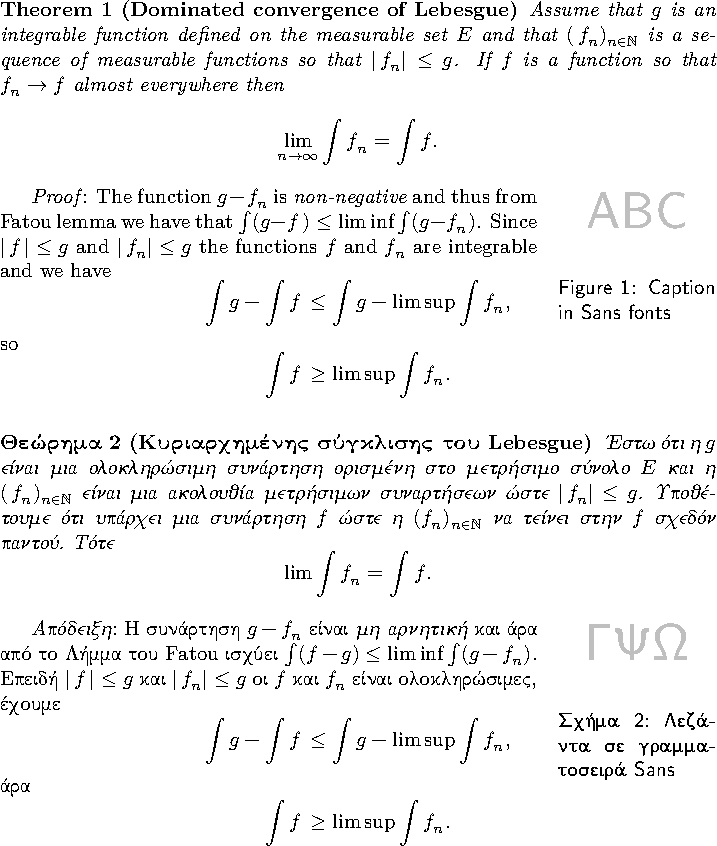
\includegraphics[scale=1.2]{fspsample-newdefault.pdf}
\end{center}
\newpage

\begin{center}
{\Large NewComputerModern fonts (old Regular weight): option \verb|olddefault|}\\[1cm] 
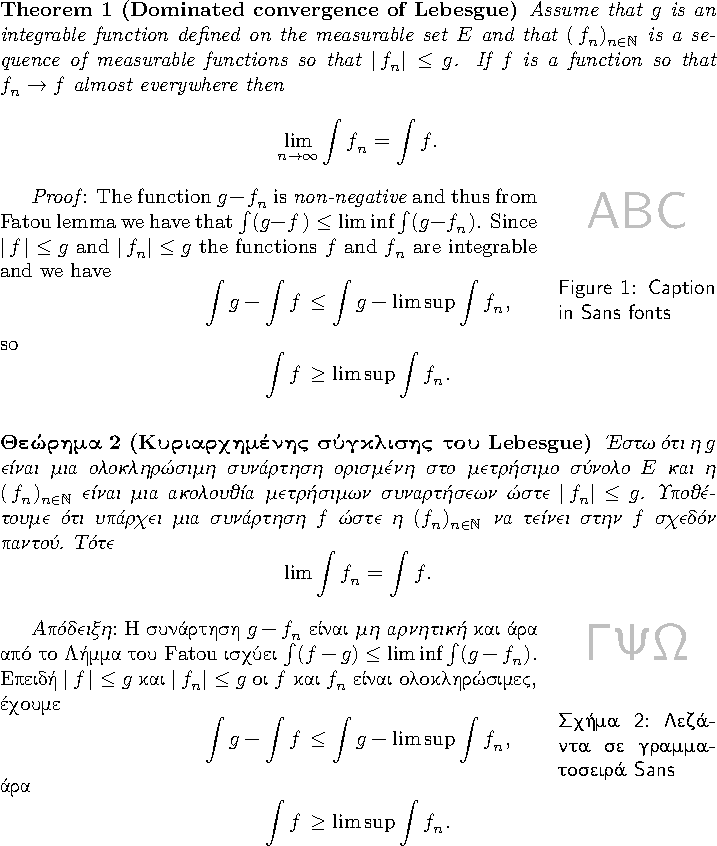
\includegraphics[scale=1.2]{fspsample-cmr.pdf}
\end{center}

\newpage
\begin{center}
{\Large NewComputerModern Sans fonts (Regular weight): option \verb|sansdefault|}\\[1cm] 
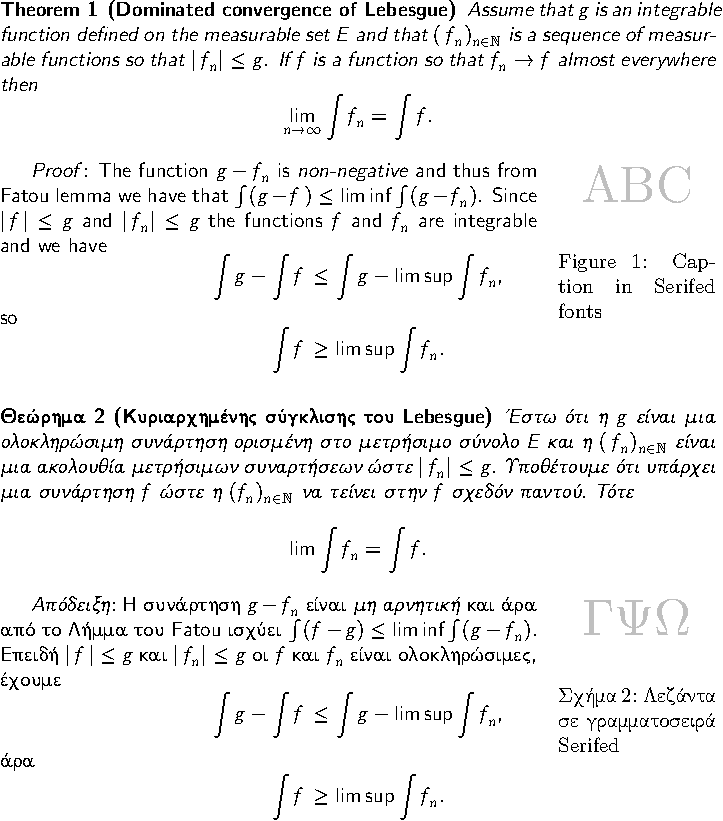
\includegraphics[scale=1.2]{fspsample-sansdefault.pdf}
\end{center}

\newpage
\begin{center}
{\Large Concrete fonts: option \verb|concrete|}\\[1cm] 
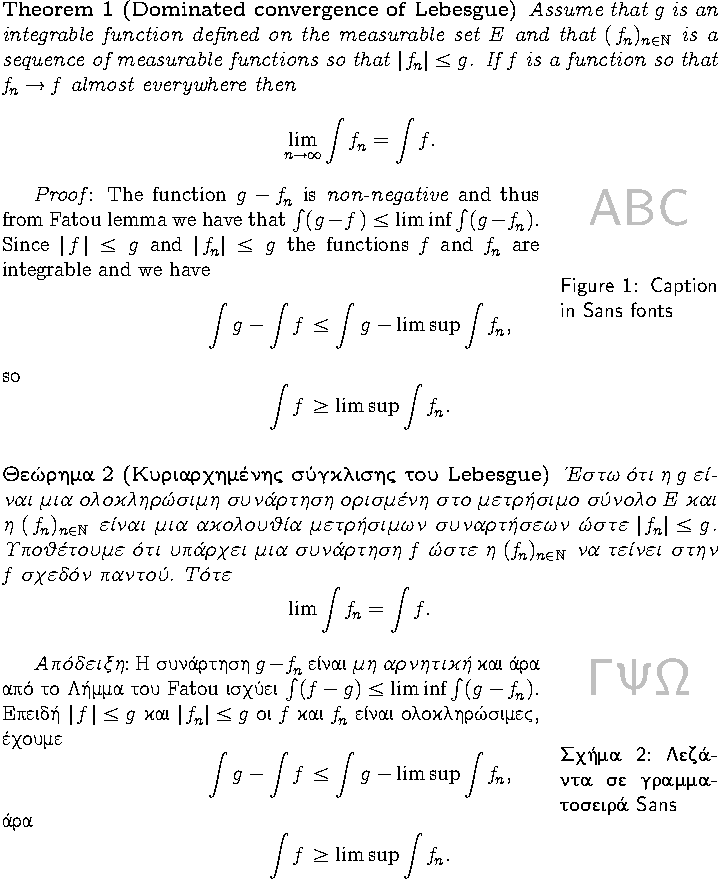
\includegraphics[scale=1.2]{fspsample-concrete.pdf}
\end{center}
\newpage

\begin{center}
{\Large EB-Garamond and Garamond-Math fonts: option \verb|ebgaramond|}\\[1cm] 
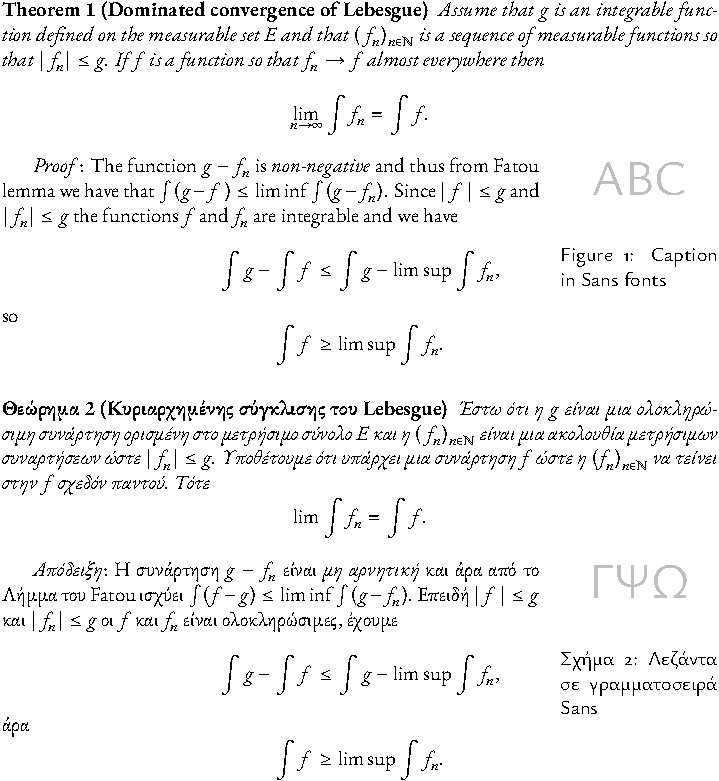
\includegraphics[scale=1.2]{fspsample-ebgaramond.pdf}
\end{center}

\newpage

\begin{center}
{\Large Erewhon and Erewhon-Math fonts: option \verb|erewhon|}\\[1cm] 
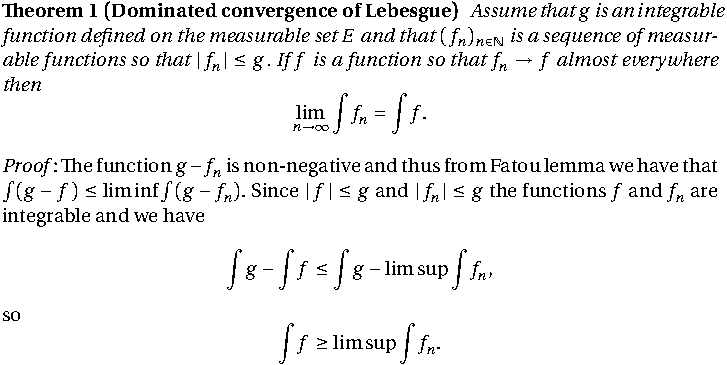
\includegraphics[scale=1.2]{fspsample-erewhon.pdf}
\end{center}

\newpage


\begin{center}
{\Large Concrete fonts and Euler-Math: option \verb|euler|}\\[1cm] 
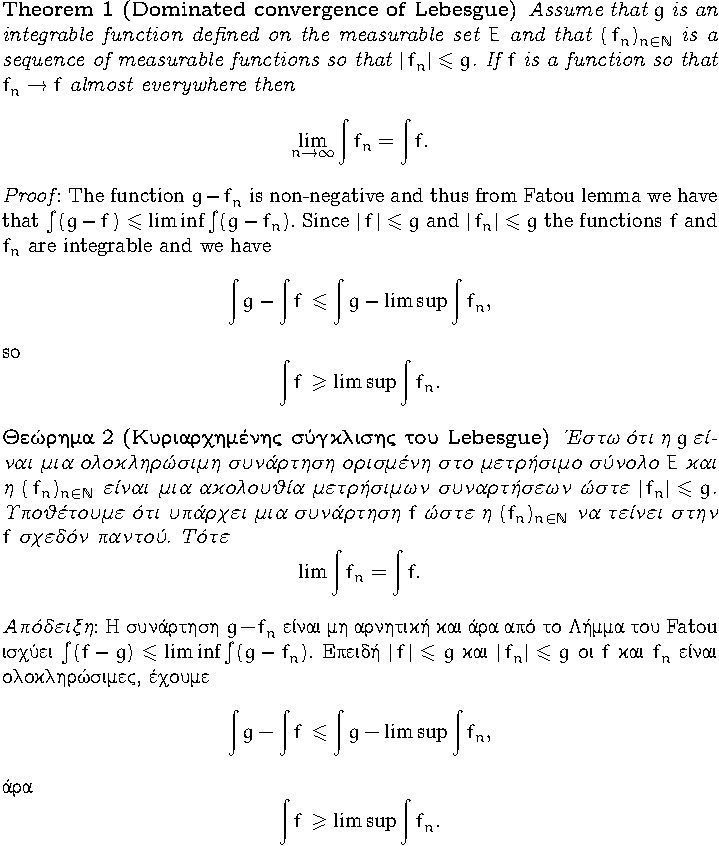
\includegraphics[scale=1.2]{fspsample-euler.pdf}
\end{center}

\newpage

\begin{center}
{\Large Fira fonts: option \verb|fira|}\\[1cm] 
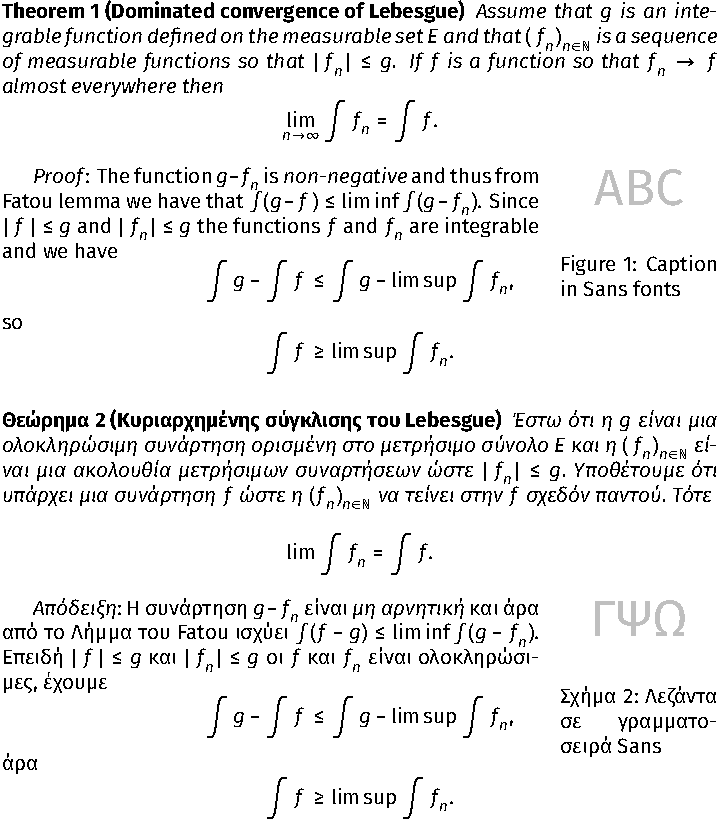
\includegraphics[scale=1.2]{fspsample-fira.pdf}
\end{center}

\newpage

\begin{center}
{\Large GFSArtemisia and Stix2Math fonts: option \verb|gfsartemisia|}\\[1cm] 
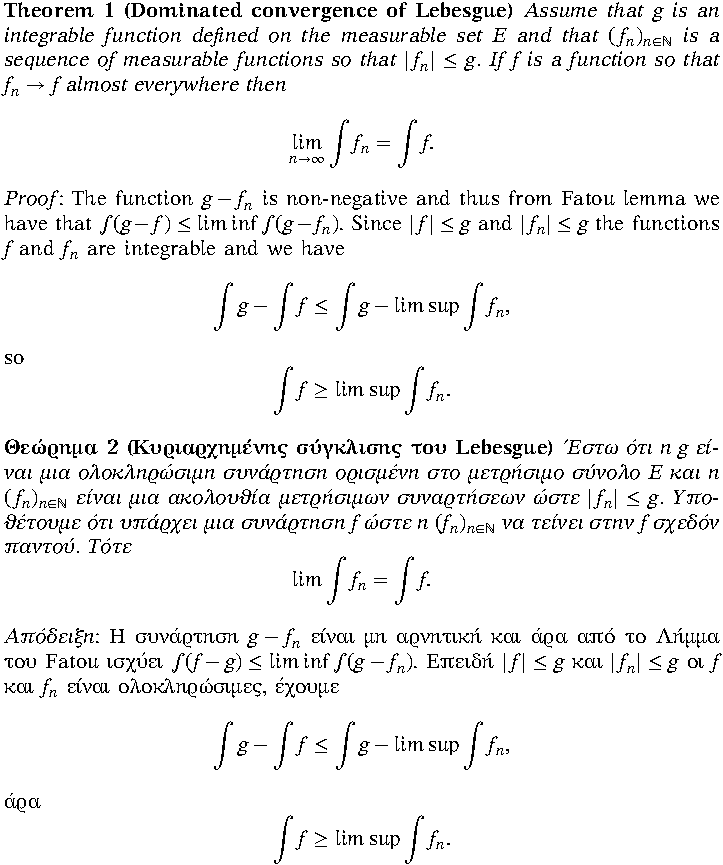
\includegraphics[scale=1.2]{fspsample-gfsartemisia.pdf}
\end{center}

\newpage

\begin{center}
{\Large GFSDidotClassic, GFSPorson Italic, and Garamond-Math fonts: option \verb|gfsdidotclassic|}\\[1cm] 
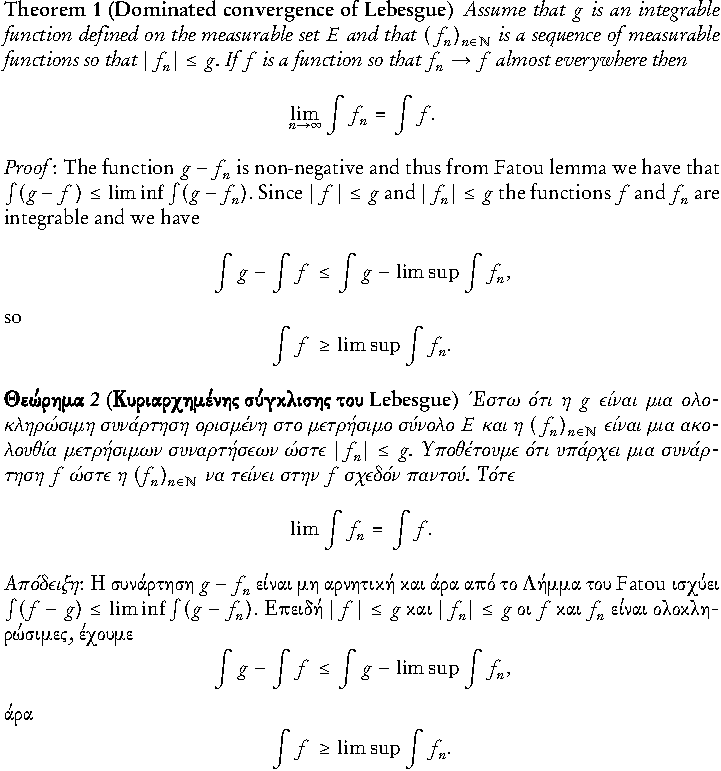
\includegraphics[scale=1.2]{fspsample-gfsdidotclassic.pdf}
\end{center}

\newpage

\begin{center}
{\Large GFSDidot and NewCMMath-Book: option \verb|gfsdidot|}\\[1cm] 
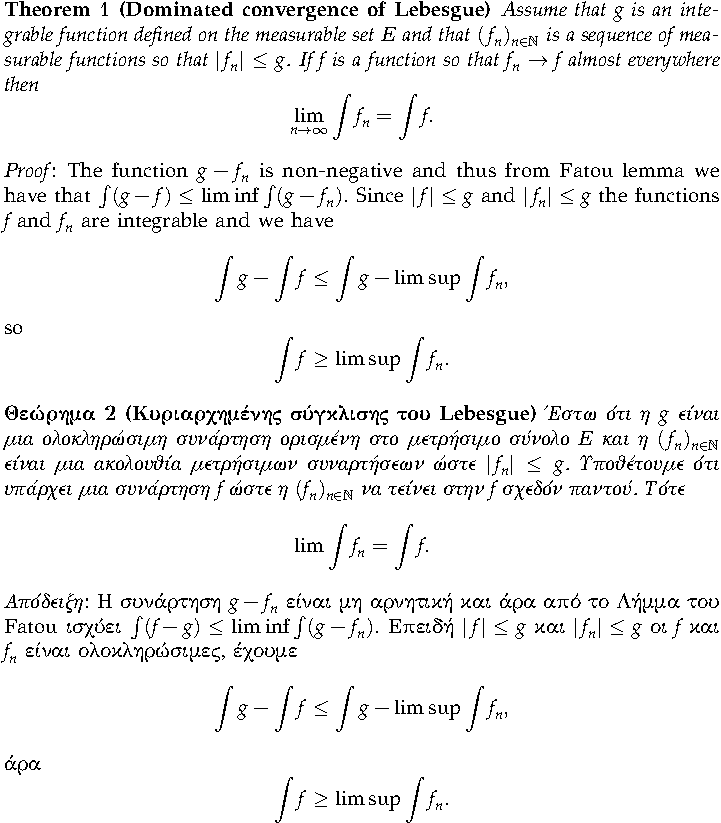
\includegraphics[scale=1.2]{fspsample-gfsdidot.pdf}
\end{center}

\newpage

\begin{center}
{\Large GFSNeohellenic and GFSNeohellenic-Math: option \verb|gfsneohellenic|}\\[1cm] 
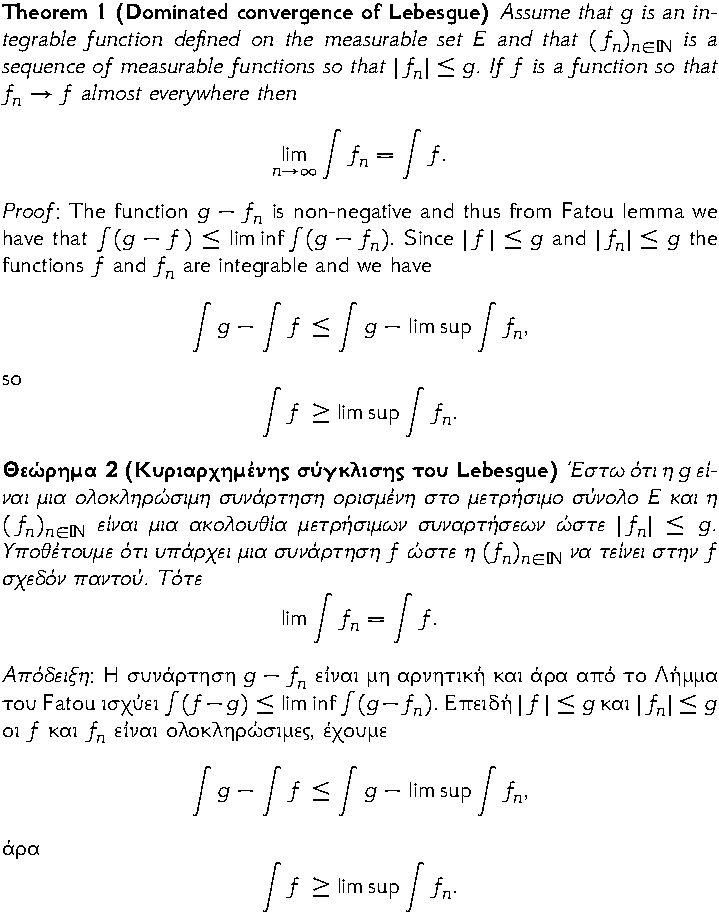
\includegraphics[scale=1.2]{fspsample-gfsneohellenic.pdf}
\end{center}

\newpage

\begin{center}
{\Large Kerkis and texgyrebonum-math: option \verb|kerkis|}\\[1cm] 
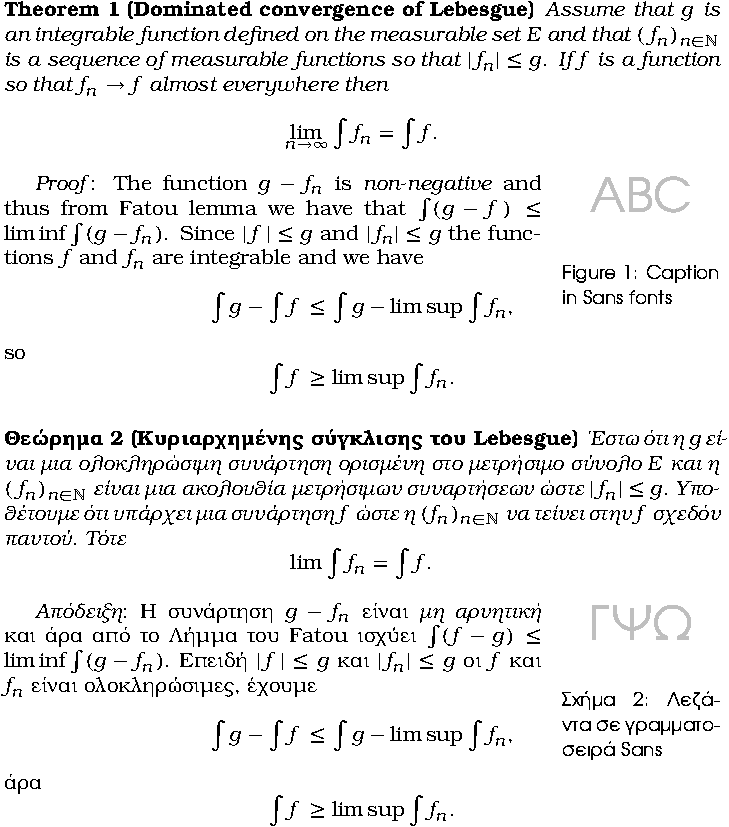
\includegraphics[scale=1.2]{fspsample-kerkis.pdf}
\end{center}



\newpage

\begin{center}
{\Large Libertinus and LibertinusMath: option \verb|libertinus|}\\[1cm]
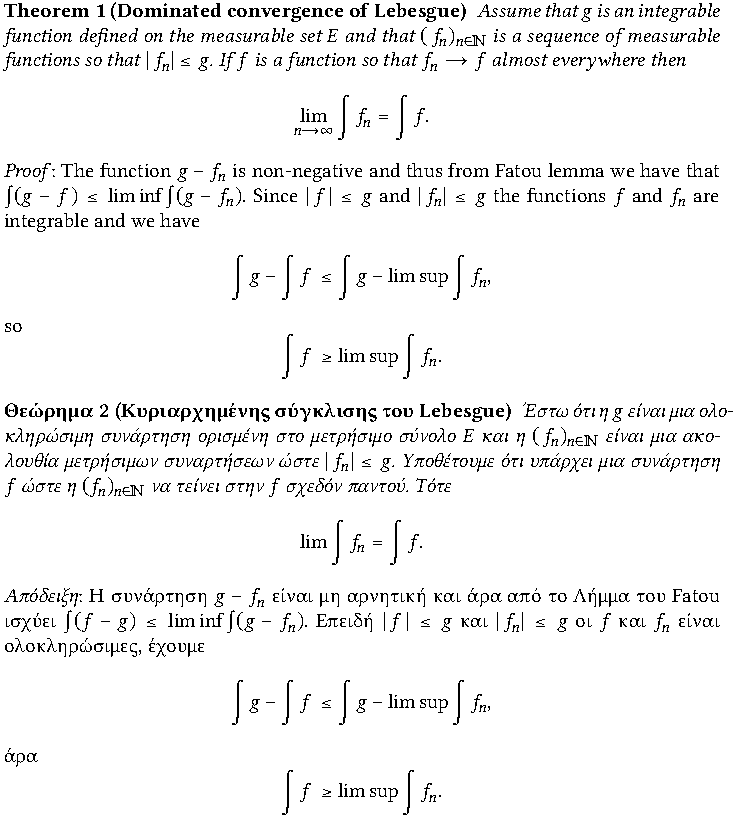
\includegraphics[scale=1.2]{fspsample-libertinus.pdf}
\end{center}



\newpage

\begin{center}
{\Large OldStandard fonts with Garamond-Math: option \verb|oldstandard|}\\[1cm] 
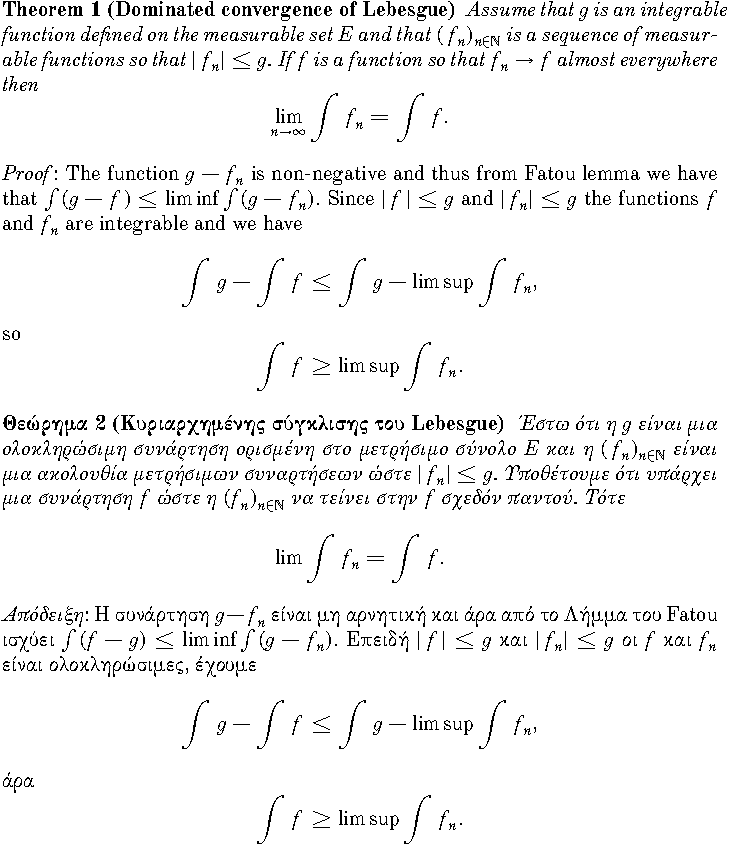
\includegraphics[scale=1.2]{fspsample-oldstandard.pdf}
\end{center}

\newpage


\begin{center}
{\Large Stix2 and Stix2Math: option \verb|stixtwo|}\\[1cm] 
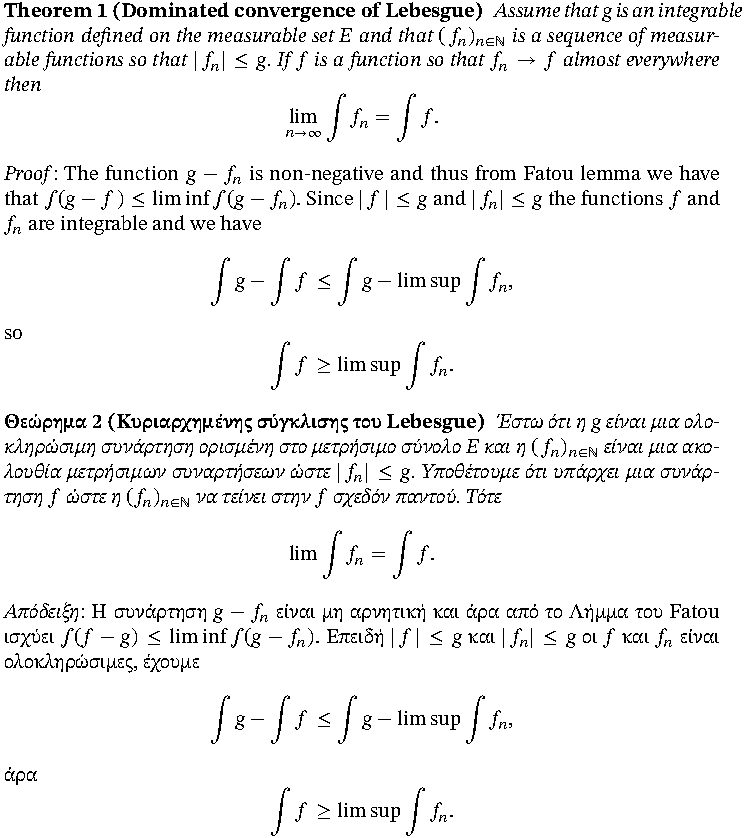
\includegraphics[scale=1.2]{fspsample-stixtwo.pdf}
\end{center}

\newpage

\begin{center}
{\Large Talos and NewCMMath-Book: option \verb|talos|}\\[1cm] 
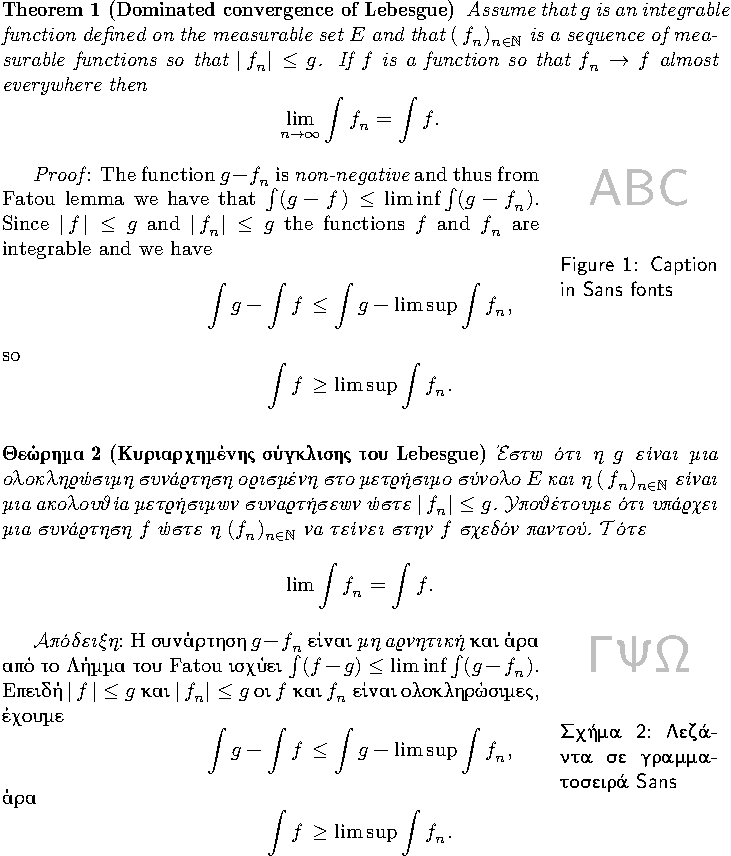
\includegraphics[scale=1.2]{fspsample-talos.pdf}
\end{center}


\newpage

\begin{center}
{\Large FreeSerifb and Stix2Math: option \verb|times|}\\[1cm] 
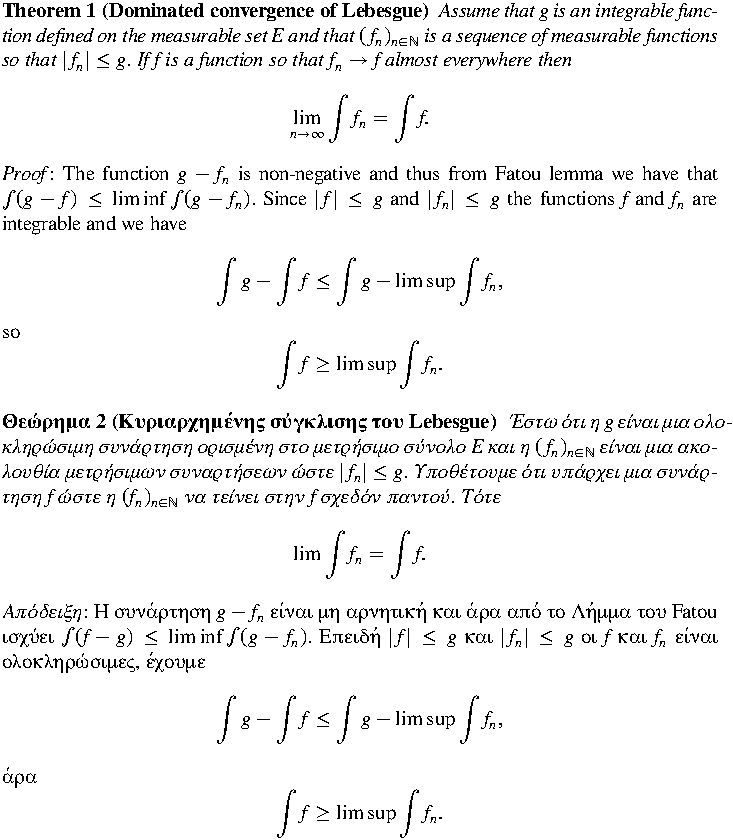
\includegraphics[scale=1.2]{fspsample-times.pdf}
\end{center}

\newpage

\begin{center}
{\Large XCharter and XCharter-Math: option \verb|xcharter|}\\[1cm] 
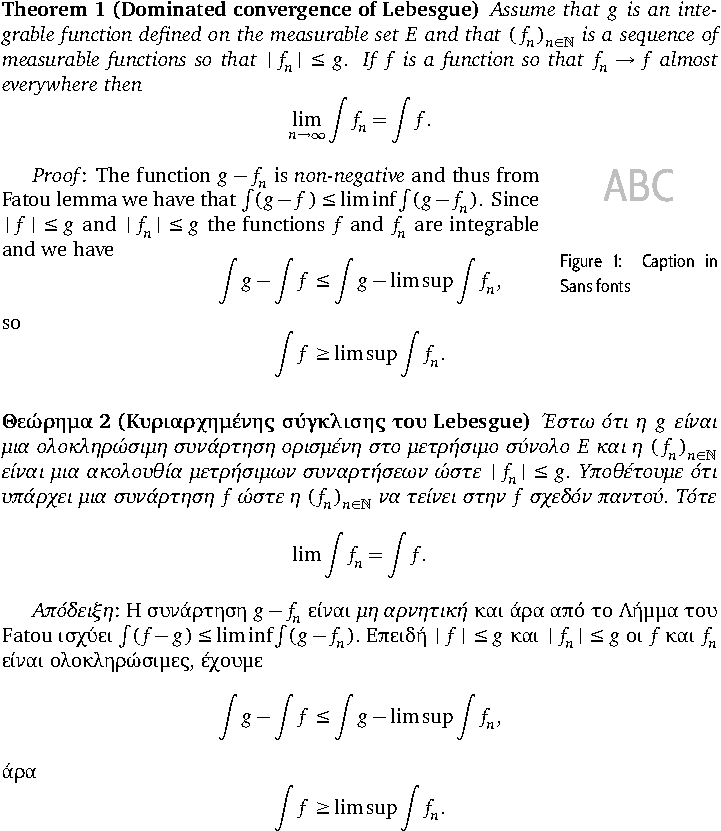
\includegraphics[scale=1.2]{fspsample-xcharter.pdf}
\end{center}



\appendix

\chapter{Ancient Greek Numbers}
The following table lists the commands and the symbol produced for the Unicode range
\texttt{u10140--u1018E}.
\begin{center}\enlargethispage{1cm}
  \begin{supertabular}{|l|l||l|l|}
    \hline
\verb|\atticonequarter|          & \atticonequarter              &\verb|\hermionianfifty|           & \hermionianfifty        \\ \hline   
\verb|\atticonehalf|              & \atticonehalf                &\verb|\thespianfifty|             & \thespianfifty             \\ \hline
\verb|\atticonedrachma|           & \atticonedrachma             &\verb|\thespianonehundred|        & \thespianonehundred        \\ \hline
\verb|\atticfive|                 & \atticfive                   &\verb|\thespianthreehundred|      & \thespianthreehundred      \\ \hline
\verb|\atticfifty|                & \atticfifty                  &\verb|\epidaurianfivehundred|     & \epidaurianfivehundred     \\ \hline
\verb|\atticfivehundred|          & \atticfivehundred            &\verb|\troezenianfivehundred|     & \troezenianfivehundred     \\ \hline
\verb|\atticfivethousand|         & \atticfivethousand           &\verb|\thespianfivehundred|       & \thespianfivehundred       \\ \hline
\verb|\atticfiftythousand|        & \atticfiftythousand          &\verb|\carystianfivehundred|      & \carystianfivehundred      \\ \hline
\verb|\atticfivetalents|          & \atticfivetalents            &\verb|\naxianfivehundred|         & \naxianfivehundred         \\ \hline
\verb|\attictentalents|           & \attictentalents             &\verb|\thespianonethousand|       & \thespianonethousand       \\ \hline
\verb|\atticfiftytalents|         & \atticfiftytalents           &\verb|\thespianfivethousand|      & \thespianfivethousand      \\ \hline
\verb|\atticonehundredtalents|    & \atticonehundredtalents      &\verb|\delphicfivemnas|           & \delphicfivemnas           \\ \hline
\verb|\atticfivehundredtalents|   & \atticfivehundredtalents     &\verb|\stratianfiftymnas|         & \stratianfiftymnas         \\ \hline
\verb|\atticonethousandtalents|   & \atticonethousandtalents     &\verb|\greekonehalfsign|          & \greekonehalfsign          \\ \hline
\verb|\atticfivethousandtalents|  & \atticfivethousandtalents    &\verb|\greekonehalfsignalt|       & \greekonehalfsignalt       \\ \hline
\verb|\atticfivestaters|          & \atticfivestaters            &\verb|\greektwothirdssign|        & \greektwothirdssign        \\ \hline
\verb|\attictenstaters|           & \attictenstaters             &\verb|\greekthreequarterssign|    & \greekthreequarterssign    \\ \hline
\verb|\atticfiftystaters|         & \atticfiftystaters           &\verb|\greekyearsign|             & \greekyearsign             \\ \hline
\verb|\atticonehundredstaters|    & \atticonehundredstaters      &\verb|\greektalentsign|           & \greektalentsign           \\ \hline
\verb|\atticfivehundredstaters|   & \atticfivehundredstaters     &\verb|\greekdrachmasign|          & \greekdrachmasign          \\ \hline
\verb|\atticonethousandstaters|   & \atticonethousandstaters     &\verb|\greekobolsign|             & \greekobolsign             \\ \hline
\verb|\attictenthousandstaters|   & \attictenthousandstaters     &\verb|\greektwoobolssign|         & \greektwoobolssign         \\ \hline
\verb|\atticfiftythousandstaters| & \atticfiftythousandstaters   &\verb|\greekthreeobolssign|       & \greekthreeobolssign       \\ \hline
\verb|\attictenmnas|              & \attictenmnas                &\verb|\greekfourobolssign|        & \greekfourobolssign        \\ \hline
\verb|\heraleumoneplethron|       & \heraleumoneplethron         &\verb|\greekfiveobolssign|        & \greekfiveobolssign        \\ \hline
\verb|\thespianone|               & \thespianone                 &\verb|\greekmetretessign|         & \greekmetretessign         \\ \hline
\verb|\ermionianone|              & \ermionianone                &\verb|\greekkyathosbasesign|      & \greekkyathosbasesign      \\ \hline
\verb|\epidauriantwo|             & \epidauriantwo               &\verb|\greeklytrasign|            & \greeklytrasign            \\ \hline
\verb|\thespiantwo|               & \thespiantwo                 &\verb|\greekounkiasign|           & \greekounkiasign           \\ \hline
\verb|\cyrenaictwodrachmas|       & \cyrenaictwodrachmas         &\verb|\greekxestessign|           & \greekxestessign           \\ \hline
\verb|\epidauriantwodrachmas|     & \epidauriantwodrachmas       &\verb|\greekartabesign|           & \greekartabesign           \\ \hline
\verb|\troezenianfive|            & \troezenianfive              &\verb|\greekarourasign|           & \greekarourasign           \\ \hline
\verb|\troezenianten|             & \troezenianten               &\verb|\greekgrammasign|           & \greekgrammasign           \\ \hline
\verb|\troezeniantenalt|          & \troezeniantenalt            &\verb|\greektryblionbasesign|     & \greektryblionbasesign     \\ \hline
\verb|\hermionianten|             & \hermionianten               &\verb|\greekzerosign|             & \greekzerosign             \\ \hline
\verb|\messenianten|              & \messenianten                &\verb|\greekonequartersign|       & \greekonequartersign       \\ \hline
\verb|\thespianten|               & \thespianten                 &\verb|\greeksinusoidsign|         & \greeksinusoidsign         \\ \hline
\verb|\thespianthirty|            & \thespianthirty              &\verb|\greekindictionsign|        & \greekindictionsign        \\ \hline
\verb|\troezenianfifty|           & \troezenianfifty             &\verb|\nomismasign|               & \nomismasign               \\ \hline
\verb|\troezenianfiftyalt|        & \troezenianfiftyalt       & & \\  \hline
  \end{supertabular}
\end{center}


\chapter{The Aegean Numbers glyph complement}
\label{AegeanNumbers}
The following table lists the commands and the symbol produced for the Unicode range
\texttt{u10100--u1013F} and the NewComputerModern fonts.

\begin{tabular}{|c|c||c|c|}\hline
\verb|\aegeanseparator| &\aegeanseparator&             \verb|\aegeaneighthundred| &\aegeaneighthundred\\ \hline                          
\verb|\aegeanseparatordot| &\aegeanseparatordot&       \verb|\aegeanninehundred| &\aegeanninehundred\\ \hline                            
\verb|\aegeancheckmark| &\aegeancheckmark&             \verb|\aegeanonethousand| &\aegeanonethousand\\ \hline                            
\verb|\aegeanone| &\aegeanone&                         \verb|\aegeantwothousand| &\aegeantwothousand\\ \hline                            
\verb|\aegeantwo| &\aegeantwo&                         \verb|\aegeanthreethousand| &\aegeanthreethousand\\ \hline                        
\verb|\aegeanthree| &\aegeanthree&                     \verb|\aegeanfourthousand| &\aegeanfourthousand\\ \hline                          
\verb|\aegeanfour| &\aegeanfour&                       \verb|\aegeanfivethousand| &\aegeanfivethousand\\ \hline                          
\verb|\aegeanfive| &\aegeanfive&                       \verb|\aegeansixthousand| &\aegeansixthousand\\ \hline                            
\verb|\aegeansix| &\aegeansix&                         \verb|\aegeanseventhousand| &\aegeanseventhousand\\ \hline                        
\verb|\aegeanseven| &\aegeanseven&                     \verb|\aegeaneightthousand| &\aegeaneightthousand\\ \hline                        
\verb|\aegeaneight| &\aegeaneight&                     \verb|\aegeanninethousand| &\aegeanninethousand\\ \hline                          
\verb|\aegeanine| &\aegeanine&                         \verb|\aegeantenthousand| &\aegeantenthousand\\ \hline                            
\verb|\aegeanten| &\aegeanten&                         \verb|\aegeantwentythousand| &\aegeantwentythousand\\ \hline                      
\verb|\aegeantwenty| &\aegeantwenty&                   \verb|\aegeanthirtythousand| &\aegeanthirtythousand\\ \hline                      
\verb|\aegeanthirty| &\aegeanthirty&                   \verb|\aegeanfourtythousand| &\aegeanfourtythousand\\ \hline                      
\verb|\aegeanfourty| &\aegeanfourty&                   \verb|\aegeanfiftythousand| &\aegeanfiftythousand\\ \hline                        
\verb|\aegeanfifty| &\aegeanfifty&                     \verb|\aegeansixtythousand| &\aegeansixtythousand\\ \hline                        
\verb|\aegeansixty| &\aegeansixty&                     \verb|\aegeanseventythousand| &\aegeanseventythousand\\ \hline                    
\verb|\aegeanseventy| &\aegeanseventy&                 \verb|\aegeaneightythousand| &\aegeaneightythousand\\ \hline                      
\verb|\aegeaneighty| &\aegeaneighty&                   \verb|\aegeanninetythousand| &\aegeanninetythousand\\ \hline                      
\verb|\aegeanninety| &\aegeanninety&                   \verb|\aegeanweightbaseunit| &\aegeanweightbaseunit\\ \hline                      
\verb|\aegeanonehundred| &\aegeanonehundred&           \verb|\aegeanweightfirstsubunit| &\aegeanweightfirstsubunit\\ \hline              
\verb|\aegeantwohundred| &\aegeantwohundred&           \verb|\aegeanweightsecondsubunit| &\aegeanweightsecondsubunit\\ \hline            
\verb|\aegeanthreehundred| &\aegeanthreehundred&       \verb|\aegeanweightthirdsubunit| &\aegeanweightthirdsubunit\\ \hline              
\verb|\aegeanfourhundred| &\aegeanfourhundred&         \verb|\aegeanweightfourthsubunit| &\aegeanweightfourthsubunit\\ \hline            
\verb|\aegeanfivehundred| &\aegeanfivehundred&         \verb|\aegeandrymeasurefirstsubunit| &\aegeandrymeasurefirstsubunit\\ \hline      
\verb|\aegeansixhundred| &\aegeansixhundred&           \verb|\aegeanliquidmeasurefirstsubunit| &\aegeanliquidmeasurefirstsubunit\\ \hline
\verb|\aegeansevenhundred| &\aegeansevenhundred&       \verb|\aegeansecondsubunit| &\aegeansecondsubunit\\ \hline                        
            & &                                        \verb|\aegeanthirdsubunit| &\aegeanthirdsubunit\\ \hline                          
\end{tabular}



\end{document}
